\documentclass[resume]{subfiles}


\begin{document}
\section{Autres}
\subsection{Triangle de Pascal}
\begin{center}
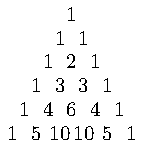
\includegraphics[scale=1,page=1]{drwg_1.pdf}
\end{center}
$$(a+b)^3=a^3+3a^2b+3ab^2+b^3$$
$$(a+b)^n=\sum_{k=0}^{n}\begin{pmatrix}
n\\k
\end{pmatrix}x^ky^{n-k}$$

$$\begin{pmatrix}
n\\ k
\end{pmatrix}=C^{n}_{k}=\frac{n!}{k!(n-k)!}$$


\end{document}